\section{Einleitung}

Das Ziel dieses Versuchs ist den Haftreibungskoeffizient $\mu_{HR}$ sowie den Gleitreibungskoeffizient $\mu_{GR}$ von unterschiedlich beschichteten Seiten eines Holz1s mit einem Holzuntergrund zu bestimmen.
\newline
Drei unterschiedliche Kräfte wirken dabei auf den Körper(siehe \autoref{fig:Kräfte}):
\begin{enumerate}
    \item Die Reibungskraft $\vec{F}_R$.
    \item Die Gewichtskraft $\vec{F}_G$.
    \item Die Normalkraft $\vec{F}_N$.
\end{enumerate}


\usetikzlibrary{angles,quotes}
\begin{figure}
    \begin{center}
        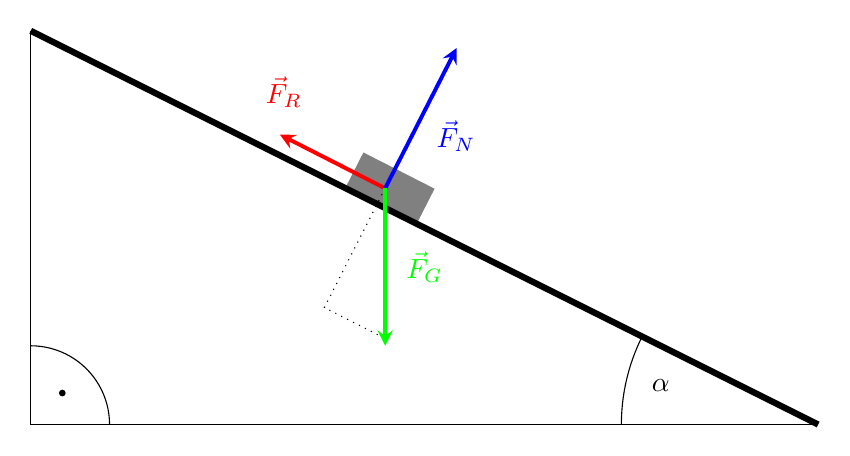
\begin{tikzpicture}
            \draw [fill, gray, rotate around={-27:(4,3)}](4,3) rectangle (5,3.5);
            \draw   (0,5) -- (0,0) -- (10,0);
            \draw [line width=0.8mm](0,5) -- (10,0);
            \draw  [domain=0:90] plot ({cos(\x)}, {sin(\x)});
            \draw [fill](0.4,0.4) circle (1pt);
            \draw [domain=153:180] plot ({10+2.5*cos(\x)}, {2.5*sin(\x)});
            \draw (8,0.5) node {$\alpha$};
            \draw [-stealth, red, line width=0.5mm, rotate around={-27:(4.5,3)}](4.5,3)--(3,3);
            \draw [red, rotate around={-27:(4.5,3)}](2.8,3.5) node {$\vec{F}_{R}$};
            \draw [-stealth, blue, line width=0.5mm, rotate around={-27:(4.5,3)}](4.5,3)--(4.5,5);
            \draw [blue, rotate around={-27:(4.5,3)}](5,4) node {$\vec{F}_{N}$};
            \draw [dotted, rotate around={-27:(4.5,3)}](4.5,3)--(4.5,1.3)--(5.4,1.3);
            \draw [-stealth, green, line width=0.5mm](4.5,3)--(4.5,1);
            \draw [green](5,2) node {$\vec{F}_{G}$};
        \end{tikzpicture}
        \caption[Kräfte]{Kräfte, die auf den Körper Wirken}
        \label{fig:Kräfte}
    \end{center}
\end{figure}

$\vec{F}_G$ lässt sich in eine zur Ebene parallele und eine senkrechte Komponente unterteilen. Die senkrechte Komponente von $\vec{F}_G$ wird durch $\vec{F}_N$ kompensiert, da $\vec{F}_N$ die selbe Kraft senkrecht zur Ebene nach oben auf den Körper ausübt wie $\vec{F}_G$ senkrecht zur Ebene nach unten. Der zur Ebene parallele teil von $\vec{F}_G$ wird als Hangabtriebskraft $\vec{F}_{HA}$ bezeichnet. $\vec{F}_R$ wirkt in Tangentialrichtung und hemmt somit die Bewegung des Körpers.
\newline
Da für $\vec{F}_{G} = m \cdot \vec{g}$ gilt, gilt ebenfalls:
\begin{subequations}
    \begin{equation}
        \abs{\vec{F}_{N}} = m \cdot g \cdot \cos{\alpha}
    \end{equation}\label{F_N}
    \begin{equation}
        \abs{\vec{F}_{HA}} = m \cdot g \cdot \sin{\alpha}
    \end{equation}\label{F_HA}
\end{subequations}
wobei $\alpha$ der Neigungswinkel der Ebene ist.
Es kann zwischen Haftreibung, Gleitreibung und Rollreibung unterschieden werden, wobei sich in diesem Versuch nur auf Haft- und Gleitreibung fokusiert wird.
\newline
Solange der Körper sich nicht bewegt wird $\vec{F}_{HA}$ komplett durch die Haftreibung $\vec{F}_{HR}$ kompensiert. $\vec{F}_{HR}$ gilt immer dann, wenn sich zwei Flächen berühren und nicht gleiten. $\vec{F}_{HR}$ kann dabei $\abs{\vec{F}_{HR}^{max}}$ nicht überschreiten:
\begin{subequations}
    \begin{align}
        \abs{\vec{F}_{HR}^{max}} &= \mu_{HR} \cdot \abs{\vec{F}_{N}} \text{ bzw.}\\
        \abs{\vec{F}_{HR}} &\leq \mu_{HR} \cdot \abs{\vec{F}_{N}}
    \end{align}
    \label{F_HR}
\end{subequations}
$\mu_{HR}$ hängt von Materialien, der Oberflächenbeschaffenheiten, sowie der Temperatur ab. \newline
Experimentell gilt für $\mu_{HR}$:
\begin{align}
    \mu_{HR} = \tan{\alpha_{max}}
    \label{MU_HR}
\end{align}
wobei $\alpha_{max}$ der größte Winkel ist, bei dem der Körper noch ruht.\newline

Sobald $\vec{F}_{HA}$ größer als $\abs{\vec{F}_{HR}^{max}}$ wird fängt der Körper an zu gleiten und es gilt die Gleitreibung $\vec{F}_{GR}$:
\begin{align}
    \abs{\vec{F}_{GR}} = \mu_{GR} \cdot \abs{\vec{F}_{N}}
    \label{F_GR}
\end{align}
$\mu_{GR}$ ist typischerweise kleiner als $\mu_{HR}$. Es wird angenommen, dass $\vec{F}_{R}$ bei einer trockenen Oberfläche unabhängig von der Geschwindigkeit des Körpers ist.\smallskip

Die resultierende Gesamtkraft $\vec{F}_{res}$ (siehe \autoref{fig:Gesamtkraft}) wird nach Newtons zweiten Axiom, dass die Kraft gleich die Masse mal die Beschleunigung ist:
\begin{align}
    \vec{F}_{res} = \vec{F}_{HA} + \vec{F}_{GR} = m \cdot \vec{a}
\end{align}

\begin{figure}[ht]
    \begin{center}
        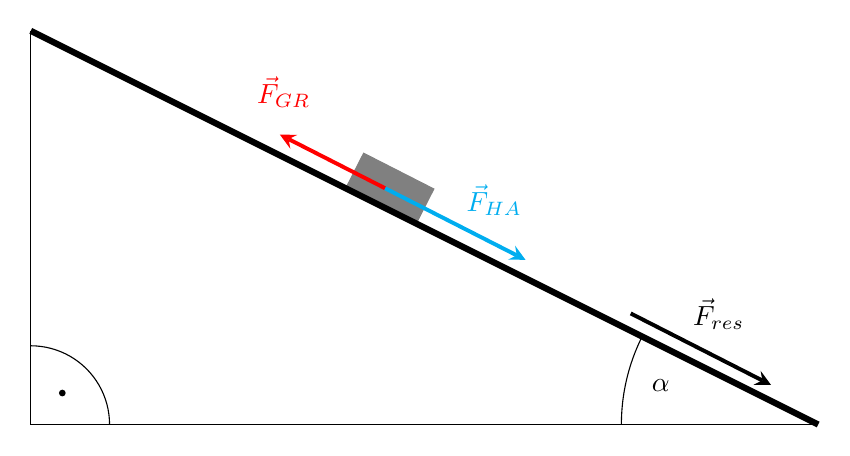
\begin{tikzpicture}
            \draw [fill, gray, rotate around={-27:(4,3)}](4,3) rectangle (5,3.5);
            \draw   (0,5) -- (0,0) -- (10,0);
            \draw [line width=0.8mm](0,5) -- (10,0);
            \draw  [domain=0:90] plot ({cos(\x)}, {sin(\x)});
            \draw [fill](0.4,0.4) circle (1pt);
            \draw [domain=153:180] plot ({10+2.5*cos(\x)}, {2.5*sin(\x)});
            \draw (8,0.5) node {$\alpha$};
            \draw [-stealth, red, line width=0.5mm, rotate around={-27:(4.5,3)}](4.5,3)--(3,3);
            \draw [red, rotate around={-27:(4.5,3)}](2.8,3.5) node {$\vec{F}_{GR}$};
            \draw [-stealth, cyan, line width=0.5mm, rotate around={-27:(4.5,3)}](4.5,3)--(6.5,3);
            \draw [cyan, rotate around={-27:(4.5,3)}](5.8,3.5) node {$\vec{F}_{HA}$};
            \draw [line width=0.5mm, -stealth, rotate around={-27:(4.5,3)}] (8,3) -- (10,3);
            \draw [rotate around={-27:(4.5,3)}](9,3.5) node {$\vec{F}_{res}$};
        \end{tikzpicture}
        \caption[Resultierende Gesamtkraft]{Aus $\vec{F}_{GR}$ und $\vec{F}_{HA}$ resultierende Gesamtkraft $\vec{F}_{res}$}
        \label{fig:Gesamtkraft}
    \end{center}
\end{figure}

Die Beschleunigung $a$ wird als Funktion der zurückgelegten Strecke $l$ und der benötigten Zeit $t_{mess}$ ausgedrückt, da gilt:
\begin{align}
    l = \frac{1}{2} a \cdot t_{mess}^2
\end{align}
Bei berücksichtigung der Formeln \autoref{F_N} und \autoref{F_GR}, ist es möglich den $\mu_{GR}$ zu bestimmen:
\begin{align}
    \mu_{GR} = \tan{a} - \frac{2\cdot l}{g \cdot t_{mess}^2 \cdot \cos{a}}
\end{align}